\documentclass[onecolumn]{emulateapj}
\usepackage{amsmath}
\usepackage{graphicx}
\usepackage{natbib}
\citestyle{aa}

\begin{document}
\title{The Hydrogen Epoch of Reionization Array Dish: Characterization with Electromagnetic Simulations}
\author{
Ewall-Wice Aaron\altaffilmark{1,2},
Abraham Neben\altaffilmark{1,2},
Nipanjana Patra\altaffilmark{5},
Thyagarajan Nithyanandan\altaffilmark{6},
Richard Bradley\altaffilmark{3,4},
Jacqueline Hewitt\altaffilmark{1,2},
Ali S. Zaki\altaffilmark{5},
Bowman Judd\altaffilmark{6},
Cheng Carina\altaffilmark{5},
Deboer David\altaffilmark{5},
Parsons Aaron\altaffilmark{5},
Venter Mariet\altaffilmark{7}
and others.
}

\altaffiltext{1}{MIT Kavli Institute for Cosmological Physics}
\altaffiltext{2}{MIT Dept. of Physics}
\altaffiltext{3}{National Radio Astronomy Obs., Charlottesville VA}
\altaffiltext{4}{Dept. of Astronomy, U. Virginia, Charlottesville VA}
\altaffiltext{5}{Astronomy Dept. U. California, Berkeley CA}
\altaffiltext{6}{School of Earth and Space Exploration, Arizona State U.,
\altaffiltext{7}{Stellenbosh}
Tempe AZ}
\begin{abstract}
Using electromagnetic simulations, we assess the spectral properties of the antenna element of the Hydrogen Epoch of Reionization Array (HERA) in order to both establish a specification for the degree of spectral structure that is permissible to sufficiently isolate foregrounds and allow a detection of the cosmological 21\,cm signal and verify direct laboratory measurements of the dish characteristics. We find that our simulations are in good agreement with field measurements. Using simulations of foregrounds, we find that the $\approx -40$\,dB response at 60\,ns of the HERA dish is sufficient to isolate the cosmological 21\,cm signal $\approx 0.2$\,$h$Mpc$^{-1}$ at $z\approx 8.5$ and obtain a high signal to noise detection of the power spectrum.
\end{abstract}
\section{Introduction}
Observations of the redshift 21\,cm radiation neutral hydrogen in the intergalactic medium (IGM) have the potential to illuminate the hitherto unobserved {\it dark ages} and {\it cosmic dawn}, revolutionizing our understanding of the first UV and X-ray sources in the universe and how their properties influenced galactic evolution (see \citet{Furlanetto:2006Review}, \citet{Morales:2010}, and \citet{Pritchard:2012} for reviews). As of now, two major experimental endeavors are underway to make a first detection of the 21\,cm signal with most focusing on the Epoch of Reionization (EoR) in which UV photons from early galaxies transformed the hydrogen in the universe from neutral to ionized. The first involves measuring the sky-averaged global signal and is being pursued by experiments such as EDGES \citep{Bowman:2010}, LEDA \citep{Greenhill:2012}, DARE \citep{Burns:2012}, SciHi \citep{Voytek:2014}, and BIGHORNS \citep{Sokolowski:2015} coming online in their planning stages or taking data. The second attempts to observe spatial  fluctuations in the 21\,cm emission using radio interferometers. As of now, a first generation of interferometry experiments are taking data in an attempt to make a first statistical detection of the power spectrum of 21\,cm brightness temperature fluctuations. These include the Giant Metrewave Telescope (GMRT)  \citep{Paciga:2013}, the Low Frequency ARray (LOFAR), \citep{VanHaarlem:2013}, the Murchison Widefield Array \citep{Tingay:2013} and the Precision Array for Probing the Epoch of Reionization (PAPER) \citep{Parsons:2010}. 

The primary obstacle to obtaining a high redshift detection of the cosmological signal through both of these methods is the existence of foregrounds that are $\sim 10^5-10^6$ times brighter. While requiring much greater sensitivity to global-signal experiments, interferometers have the advantage that these spectrally smooth foregrounds naturally avoid a significant region of $k$-space, known as the {\it EoR window}, occupying a region known as the {\it wedge} \citep{Datta:2010,Vedantham:2012,Parsons:2012,Thyagarajan:2013,Liu:2014a,Liu:2014b}, however any structure in the frequency response of the instrument has the potential to leak foregrounds into the EoR window, masking our signal. Indeed, low level spectral structures in the analogue and digital signal chains on the initial buildout of the MWA are proving to be a significant obstacle \citep{Dillon:2015b,EwallWice:2015a,Beardsley:2015b}. 

While, in principle, spectral structure in the bandpass of the instrument may be removed in calibration, simulations show that any mismodeling of emission and the primary beam, potentially below the confusion limit, will mix the significant spectral structure on long baselines into short ones, masking the signal entirely \citep{Barry:2015}. While redundant calibration \citep{Wieringa:1992,Liu:2011,Zheng:2014} is able to calibrate the independent of a detailed model of the sky, any direction-dependent chromatic structure in the primary beam of the instrument introduces additional degrees of freedom that must be modeled, potentially leading to signal loss and the introduction of spurious spectral structure due to unmodeled foregrounds in long baselines. Because of our limited knowledge of foregrounds at low-frequency and the fidelity of calibration algorithms, the only sure way of building an instrument that will guarantee a detection of the redshifted 21\,cm emission is to design it such that all spectral structure in the signal chain is limited to a finite region of delay space, well below the wedge.


The Hydrogen Epoch of Reionization Array (HERA) is an instrument currently taking first observations in the Karoo in South Africa with the ultimate goal of detecting the power spectrum of 21\,cm brightness temperature fluctuations at high signal-to-noise (SNR) \citep{Pober:2014}. A central principle in HERA's design is that it be calibration fail-safe such that a detection of the signal is guaranteed, even if the chromaticity of the instrument is not calibrated out. This paper and its companions \citep{Neben:2015b,Patra:2015,Thyagarajan:2015c} describe a multifaceted approach to establishing a stringent specification on the spectral structure permissible for HERA to be calibration fail-safe and determine to what extent its design meets these requirements. We accomplish this by establishing a spec with simulations of foregrounds \citep{Thyagarjan:2015c} and verifying that HERA primary antenna element meets this spec with reflectometry \citep{Patra:2015} and Orbcomm beam mapping \citep{Neben:2015b}. These measurements are verified with detailed electromagnetic simulations which we describe in this work. 

This paper is organized as follows. In \S~\ref{sec:Formalism} we lay out our analytic framework for describing the impact of reflections and spectral structure on foreground leakage in delay-transform power spectra. In \S~\ref{sec:Simulations} we describe our electromagnetic simulations of the HERA dish element. In \S~\ref{sec:Comparison} we compare our simulation results to direct measurements of the primary dish element and in \S~\ref{sec:Foregrounds} we apply our electromagnetic simulation results to simulations of foregrounds to determine the extent that the HERA dish's chromatic structure pollutes the EoR window and their impact on HERA's overall sensitivity. We conclude in \S~\ref{sec:Conclusion}.

\section{The Impact of Reflections on Delay-Transform Power Spectra}\label{sec:Formalism}
In this section, we show how reflections in the analogue signal path of an antenna lead to foreground contamination of the EoR window. Inuitively, any reflections in the signal path introduce sinusoidal ripples in the frequency dependent gain of the instrument. Since reflection delay is the Fourier dual to frequency, reflections at larger delays introduce ripples at higher frequencies. Isolation of the 21\,cm signal from foregrounds that are over five orders of magnitude brighter depends critically on the fact that their smoothness. Any sinusoidal frequency structure, introduced by the antenna gain will cause these foregrounds to mimic and swamp the signal unless they are brought below a level similar to the ratio between the foregrounds and the signal itself. We now derive this process in formal detail. We assume that the intensity field on the sky is given by 
\begin{equation}\label{eq:Dirac}
I({\bf \widehat{k}},f) \delta_D({\bf \hat{k}} - {\bf \hat{k}'})= \langle s({\bf \hat{k}},f)s^*({\bf \hat{k}'},f)  \rangle_t^2
\end{equation}
 where $\delta_D$ is the Dirac delta function. We imagine that the electric field as a function of time, $\widetilde{s}({\bf \widehat{k}},t)$ arrives at an arbitrary origin at time $t$ and at the various $i^{th}$ antenna elements of an interferometer at locations ${\bf x_i}$ at times $\tau_i={\bf x_i} \cdot {\bf \widehat{k}} /c$. We now consider reflections within a single dish element described by a direction dependent reflection coefficient\footnote{Ignoring reflections between multiple dish elements which we treat in Appendix~\ref{app:Reflections}}, $\widetilde{r}_i({\bf \widehat{k}},\tau)$. which re-introduce the signal at later times $\tau$. The voltage signal measured at the $i^{th}$ antenna element, $\widetilde{v}_i$, is the integral over solid angle of the convolution of the electric field entering the antenna (delayed by $\tau_i$) with $r_i({\bf \widehat{k}},\tau')$.

\begin{equation}
\widetilde{v}_i(t) = \int d \Omega \int d \tau \widetilde{r}_i({\bf \widehat{k}},\tau') \widetilde{s}({\bf \widehat{k}},t+\tau_i - \tau)
\end{equation}

 An FX (or XF) correlator measures the time-averaged product of the fourier transform of the voltage streams between the $i^{th}$ and $j^{th}$ antenna. Fourier transforming the voltage stream from the $i^{th}$ antenna we obtain
\begin{equation}
v_i(f) = \int d \Omega \int d \tau' \widetilde{r}_i({\bf \widehat{k}},\tau') s({\bf \widehat{k}},f)e^{2 \pi i f(\tau'-\tau_i)}
\end{equation}
The time averaged product between the two antennas is
\begin{equation}
V_{ij}'(f) = \left \langle v_i(f) v_j^*(f) \right \rangle_t = \int d \Omega \int d \tau \widetilde{r}_i(\tau) d \tau' \widetilde{r}^*_j(\tau')e^{2 \pi i f (\tau'-\tau) } I({\bf \widehat{k}}, f) e^{- 2 \pi i \Delta \tau_{ij}f} 
\end{equation}
where $\Delta \tau_{ij} = \tau_i-\tau_j = ({\bf x_i - x_j}) \cdot {\bf \widehat{k}}/c$. We eliminated one of the solid angle integrals using equation~\ref{eq:Dirac}. 

Defining ${\bf u}_{ij} = f ({\bf x}_i-{\bf x}_j)/c$, we obtain,
 %HERA's primary antenna element consists of a sleeved dipole element suspended 5\,m above the focus of a 14\,m diameter parabolic dish (Fig.~\ref{fig:Dish}).
.
%\begin{figure}
%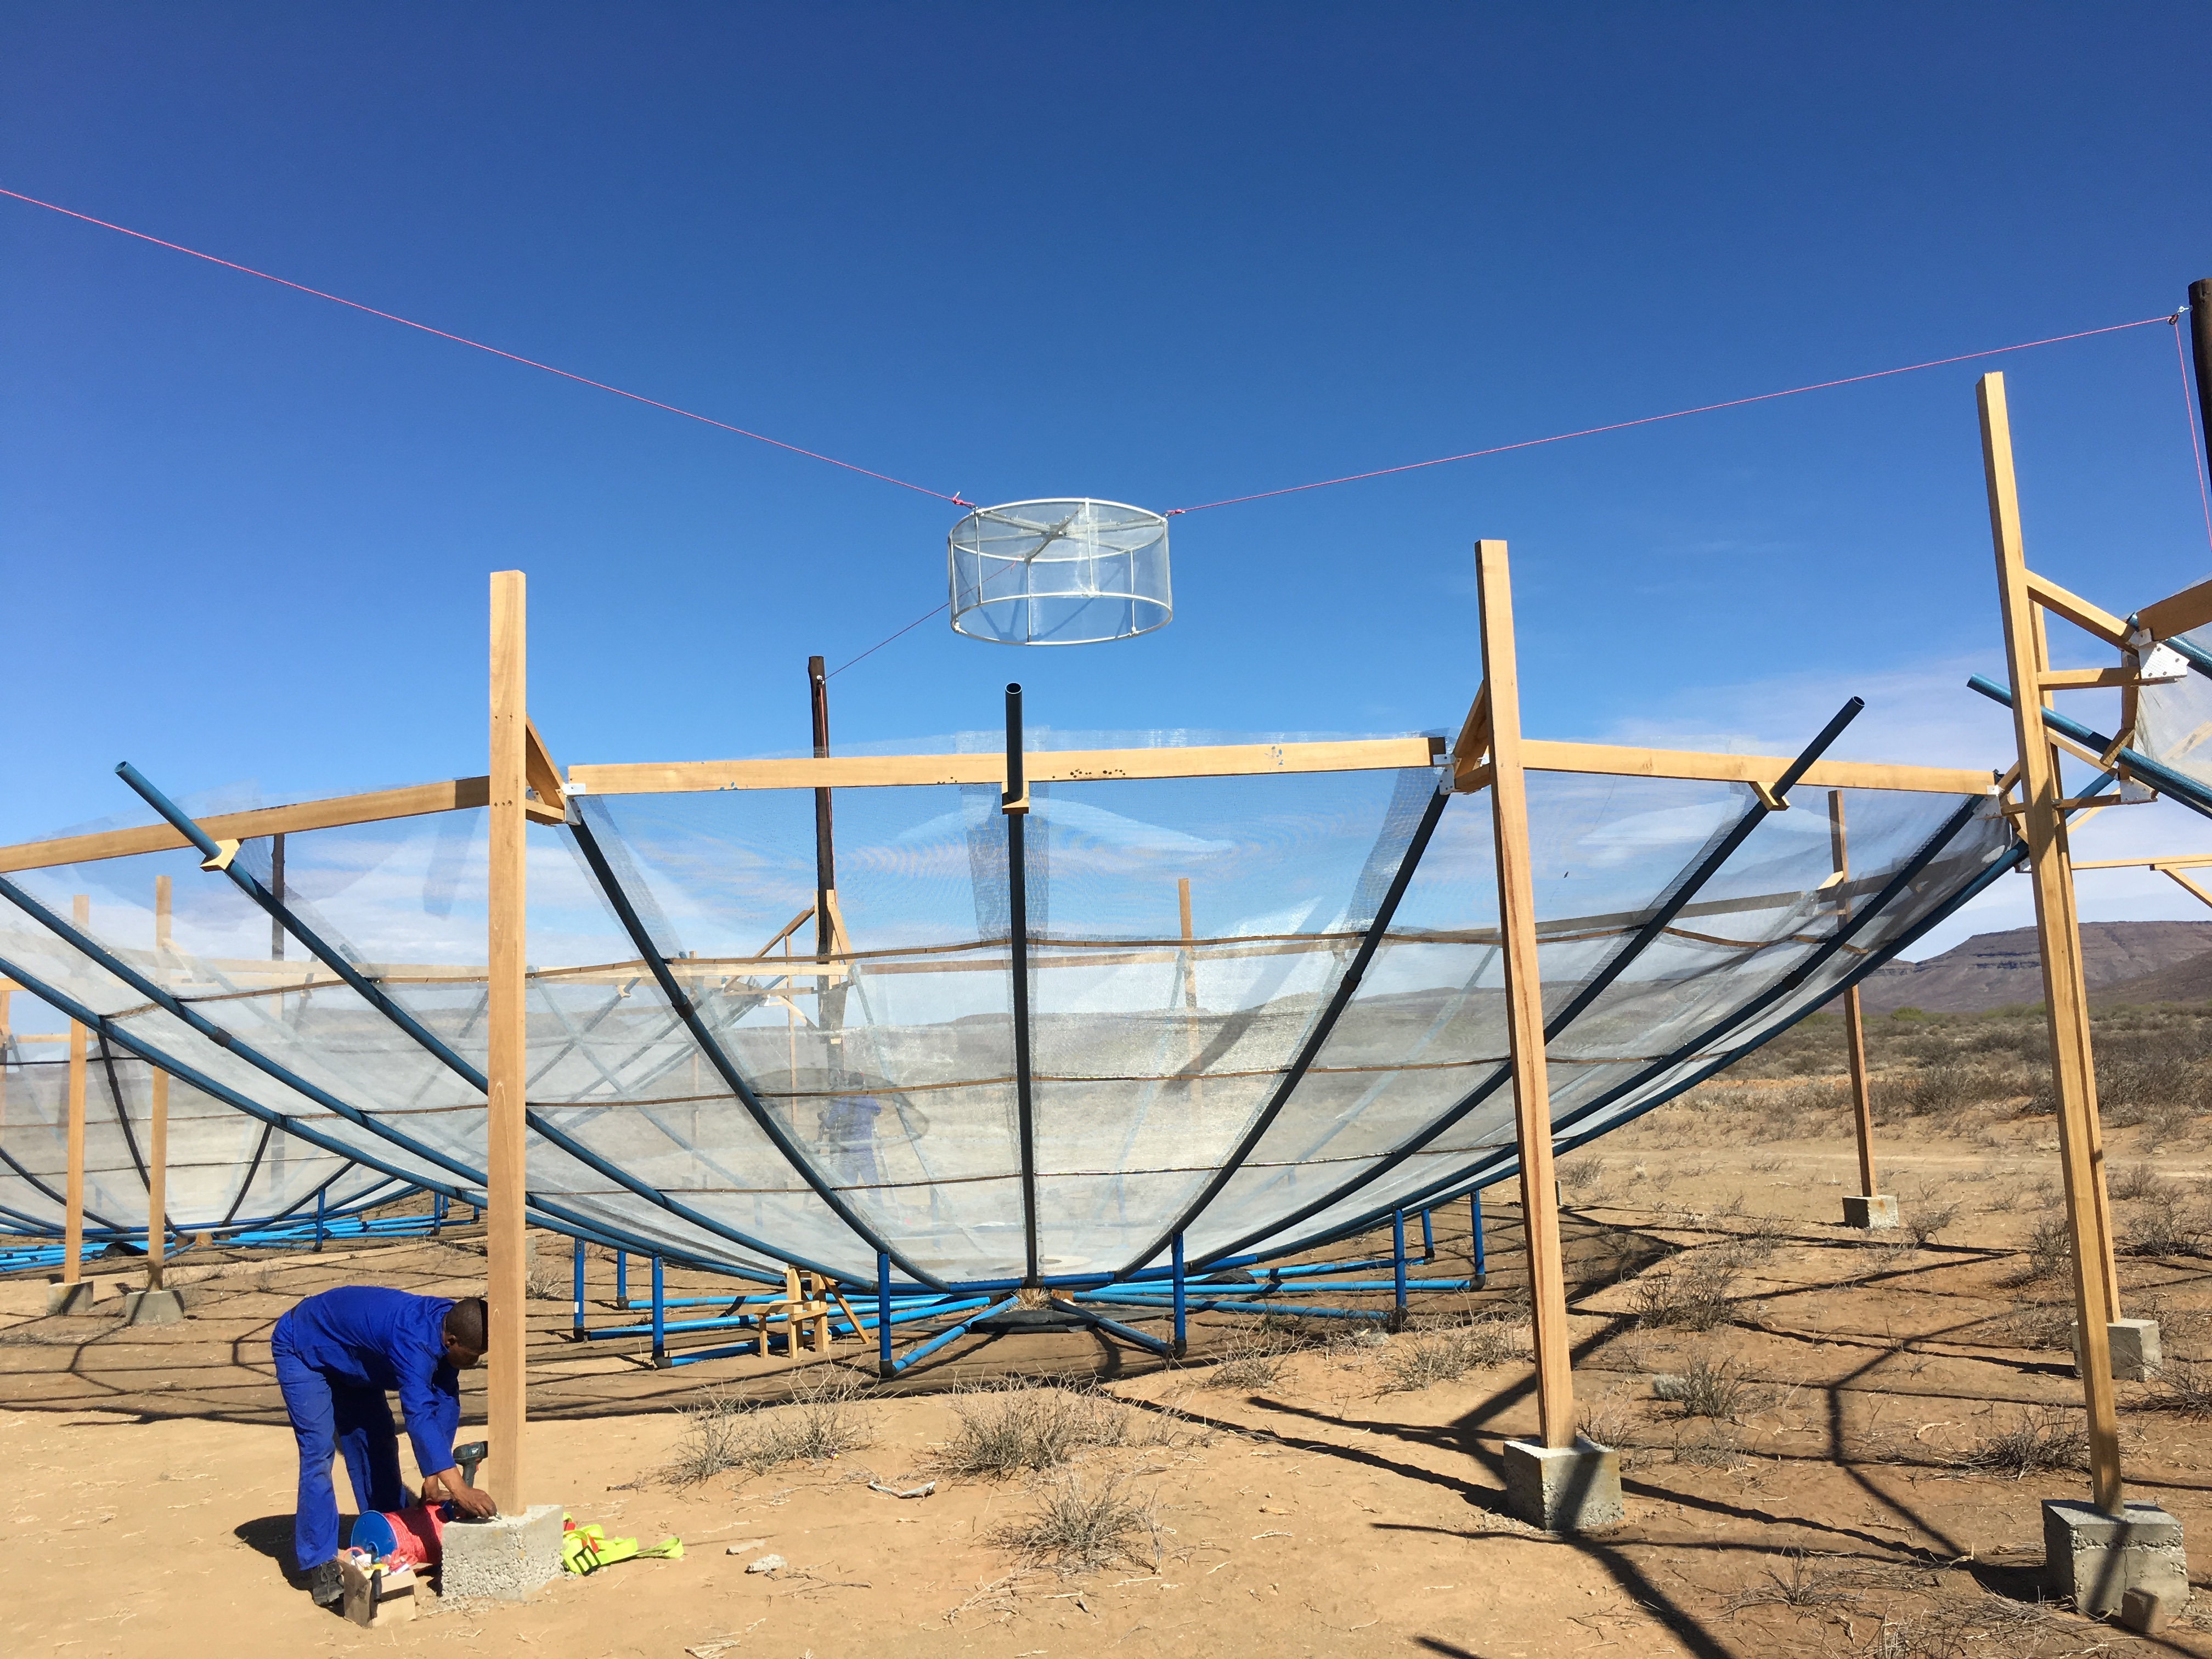
\includegraphics[width=.5\textwidth]{figures/DishSA.png}
%\caption{The HERA primary antenna element-one of 19 undergoing currently taking the first observations in the Karoo in South Africa. The antenna consists of a sleeved dipole suspended within a 2\,m diameter skirt, five meters above the ground at the focal point of a 14\,m diameter dish.}\label{fig:Dish}
%\end{figure}

% We show in Appendix~\ref{app:Reflections} that if an astronomical radio signal with time dependence at the location of the feed, $s({\bf \widehat{k}},t)$, experience reflections within the dish such that the voltage recorded in the feed is 
 
 

Than the resulting visibilities obtained by cross correlating antenna $i$ and antenna $j$ are given by 
\begin{equation}
V'_{ij}(f) =  \int d \Omega r_i({\bf \widehat{k}},f) r^*_j({\bf \widehat{k}},f)  I(f,{\bf \widehat{s}})e^{2 \pi i {\bf u}_{ij} \cdot {\bf \widehat{k}}},
\end{equation}
where ${\bf u}_{ij} = ({\bf x}_i - {\bf x}_j ) f/c$ to use the usual $uv$ notation of interferometry. $r_i({\bf \hat{k}},f)$ is the inverse fourier transform of the reflection response of the dish, hence we see that the reflection response is precisely the Fourier dual to the Dish's frequency domain voltage beam. Setting a specification on reflections is hence equivalent to setting a specification on spectral smoothness. 

In order to separate spectrally smooth foregrounds from our signal, we expect to use the {\it delay transform} over frequency, defined as \citep{Parsons:2012}
\begin{equation}
\widetilde{V}_{ij}(\tau) = \int d f e^{-2 \pi i \tau f} V_{ij}(f)
\end{equation}
Applying this to equation~\ref{eq:}
\begin{equation}
\widetilde{V}_{ij}'(\tau) = \sum_{m,n} \widetilde{V}_{ij,FG}^{mn}(\tau - \Delta \tau_{mn}) + \widetilde{V}_{ij,21}^{mn}(\tau - \Delta \tau_{mn})
\end{equation}
where $V_{ij}^{mn}$ is a visibility resulting from the effective primary beam, $R_{ij}({\bf \widehat{k}},\Delta \tau_{mn})$, at delay $\Delta \tau_{mn}$ induced by the reflections.
\begin{equation}
V_{ij}^{mn} = \int d \Omega R_{ij}({\bf \widehat{s}},\Delta \tau_{mn}) I(f,{\bf \widehat{s}})e^{2 \pi i {\bf u}_{ij} \cdot {\bf \widehat{s}}}
\end{equation}
The delay transform power spectrum estimate, $\widehat{P}$, is proportional to $|\widetilde{V}_{ij}'|^2$, hence 
\begin{align}\label{eq:Reflections}
\widehat{P} & \propto |\widetilde{V}_{ij,FG}(\tau)|^2 + |\widetilde{V}_{ij,21}(\tau)|^2 + 2 \text{Re}(\widetilde{V}_{ij,21}(\tau)\widetilde{V}_{ij,FG}^*(\tau)) \nonumber \\
&+ \sum_{|\Delta \tau_{mn}| > 0} 2 \text{Re} \left[   \widetilde{V}^*_{ij} (\tau) \widetilde{V}^{mn}_{ij} (\tau - \Delta \tau_{mn})  \right] \nonumber \\
&+ \sum_{\substack{|\Delta \tau_{op}|>0\\|\Delta \tau_{mn}|>0}} \widetilde{V}^{mn}_{ij} (\tau - \Delta \tau_{mn}) \widetilde{V}^{op*}_{ij}(\tau - \Delta \tau_{op})
\end{align}
In the absence of reflections, only the top line of equation~\ref{eq:Reflections} would enter the delay power spectrum estimate. The following lines involve the translation of the signal (including foregrounds and signal) out to the delay of each reflection and weighted by the effective primary beam of the reflection. Since each translated visibility is intrinsically $\sim 10^6$ times brighter than the signal, any reflection with a delay large enough to place it within the EoR window, must be sufficiently attenuated by $R_{ij}({\bf \widehat{k}},\Delta \tau_{mn})$.% The precise degree of attenuation is determined in \citep{Thyagarajan:2015c} using simulations of foregrounds and noise and sets the spec for our antenna.

To get a better idea for what spec this sets on the voltage response of our dish we examine, in more detail, the case where $r_0$ at ($\tau=0$) is significantly greater than the other coefficients as we might expect for a dish with a relatively smooth gain. Than we can approximate equation \ref{eq:Reflections} to linear order in $r_i$,
\begin{equation}
\widetilde{V}_{ij}'(\tau) \approx \widetilde{V}_{ij} + \sum_{m>0} \widetilde{V}_{ij}^{m0} (\tau -  \tau_m)
\end{equation}



If we make the assumption that the beam can be factored into a frequency dependent and frequency dependent term, $r_i({\bf \widehat{k}},\tau) = a_i({\bf \widehat{k}}) g_i(\tau)$ than we have
\begin{equation}
\widetilde{V}_{ij}' \approx \widetilde{V}_{ij}(\tau) + \sum_{m>0} r_m \widetilde{V}_{ij}(\tau - \tau_m)
\end{equation}
 Hence, for a delay response dominated by the $0$-delay mode, as we might expect in an antenna element with smooth gain, the delay transformed visibilities are effectively convolved with the {\it voltage response}, not the square of the voltage response as we might naively expect. A more compact writing the impact of the spectral structure of a separable beam on foregrounds would be
 \begin{equation}
 	\widetilde{V}_{ij}'(\tau) = \left[ (g_i \star g_j^*) \star \widetilde{V}_{ij}\right](\tau)
 \end{equation}
 As a result, one should compare the amplitude of the voltage delay response of the antenna with the ratio between foregrounds and signal when 


 In this paper, we study $r_i({\bf \widehat{k}},\Delta \tau)$ for the HERA antenna element to verify that it both meets the spec and agrees with direct measurements of the antenna element with refelctometry \citep{Patra:2015} and Orbcomm measurements \citep{Neben:2015b}. We also explore the implications of the performance of $r_i({\bf \widehat{k}},\tau)$ on the scientific bottom line for EoR experiments, using the Fisher Matrix Formalism. 

\section{Electromagnetic Simulations of the HERA dish element}\label{sec:Simulations}
In Fig.~\ref{fig:SimulationSetup} we show the geometery of the electromagnetic simulation. {\bf Rich: fill in the details here}
\begin{figure}


\subsection{The Simulations}
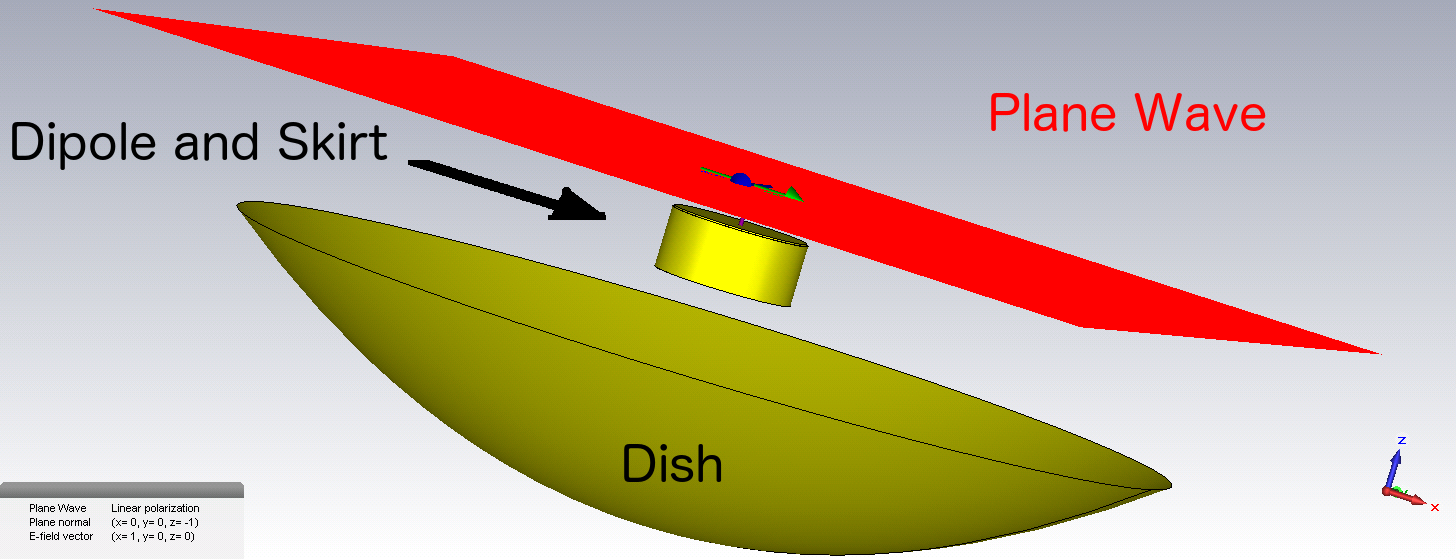
\includegraphics[width=.5\textwidth]{figures/One_dish_Pfeed_render_pw_0deg.png}
\caption{A rendering of our time domain simulation at $t=0$, demonstrating the geometry and setup of our electromagnetic simulation. The plane wave is started just above the feed (red plane).}\label{fig:SimulationSetup}
\end{figure}

\begin{figure*}
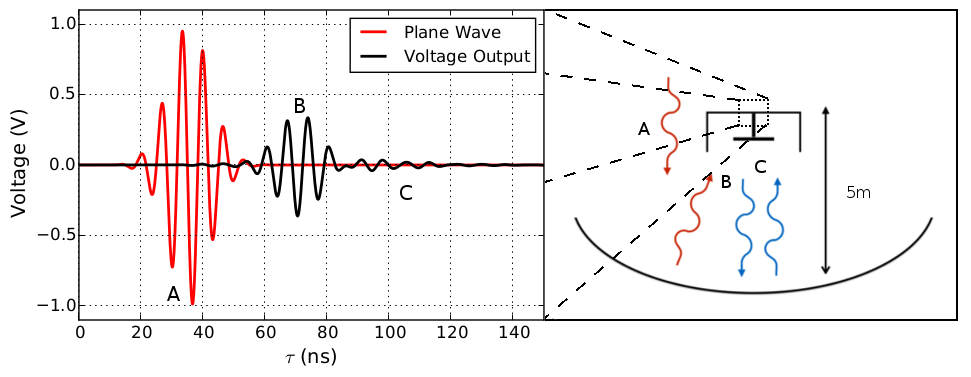
\includegraphics[width=\textwidth]{figures/SimulationIllustration.png}
\caption{An illustration of our simulation products and their origin in the HERA antenna geometry. A plane wave is injected from above the feed (red line). The amplitude of the electric field of the plane wave at output of the feed along with the voltage at the feed terminal outputs is recorded (black line). The feed in our simulation is situated $5$\,m above the bottom of the dish, hence there is a $\approx 30$\,ns delay between when the plane wave passes the terminal for the first time (A) and when it is first absorbed in the dipole (B), leading to the voltage response. Of concern to 21\,cm experiments are the subsequent reflections between the feed and the dish (C) which can lead to large delay contamination of the EoR window.}
\label{fig:Simulation}
\end{figure*}
\subsection{Deconvolving the Response Function}
In our simulation, we obtain the voltage at the feed output as a function of time which we will call $v_{out}(t)$. It is related to the input lane wave through the equation 
\begin{equation}
v_{out}(t,\theta=0) = \sum_n r_n(\theta=0) v_{in}(t - \tau_n,\theta=0),
\end{equation}
which is essentially a convolution in time of $r_n(\theta=0)$ with the input plane wave. We may undo this convolution by taking a discrete Fourier transform of both $v_{out}$ and $v_{in}$ in time, dividing them in Fourier space, and taking an inverse DFT back. Our simulation output is sampled at even time intervals so we may use and FFT. 
\begin{equation}
\widehat{{\bf r}}(\theta=0) = \boldsymbol{\mathcal{F}}^{-1} \left[ \frac{\boldsymbol{\mathcal{F}} {\bf v_{out}}(\theta=0)}{{\bf v_{in}}(\theta=0)} \right] 
\end{equation}
where ${\bf \mathcal{F}}$ is the Fourier transform matrix for a 1d vector of length $N$. 
\begin{equation}
\boldsymbol{\mathcal{F}}_{mn} = e^{2 \pi i m n /N}
\end{equation}
In Fig.~\ref{fig:FrequencyDomain} we show the amplitude of the Fourier transform of our Gaussian input, centered at $150$\,MHz along with the voltage response. Since our input is band limited between $\approx 20$ and $280$\,MHz, the direct ratio of our voltage response and input wave is dominated by numerical noise outside of this range. We eliminate these numerical artifacts by multiplying our ratio by a Hamming window between $50$\,MHz and $250$\,MHz and set our estimate to zero elsewhere. From a physical standpoint, this is sensible since 21\,cm experiments only observe a limited bandwidth. PAPER's correlator, which will initially serve as the HERA backend samples over a $100$\,MHz instantaneous freqeuency interval. Hence analogue filtering is applied to limit the incoming signal within a finite bandwidth and prevent aliasing.

\begin{figure}[h!]
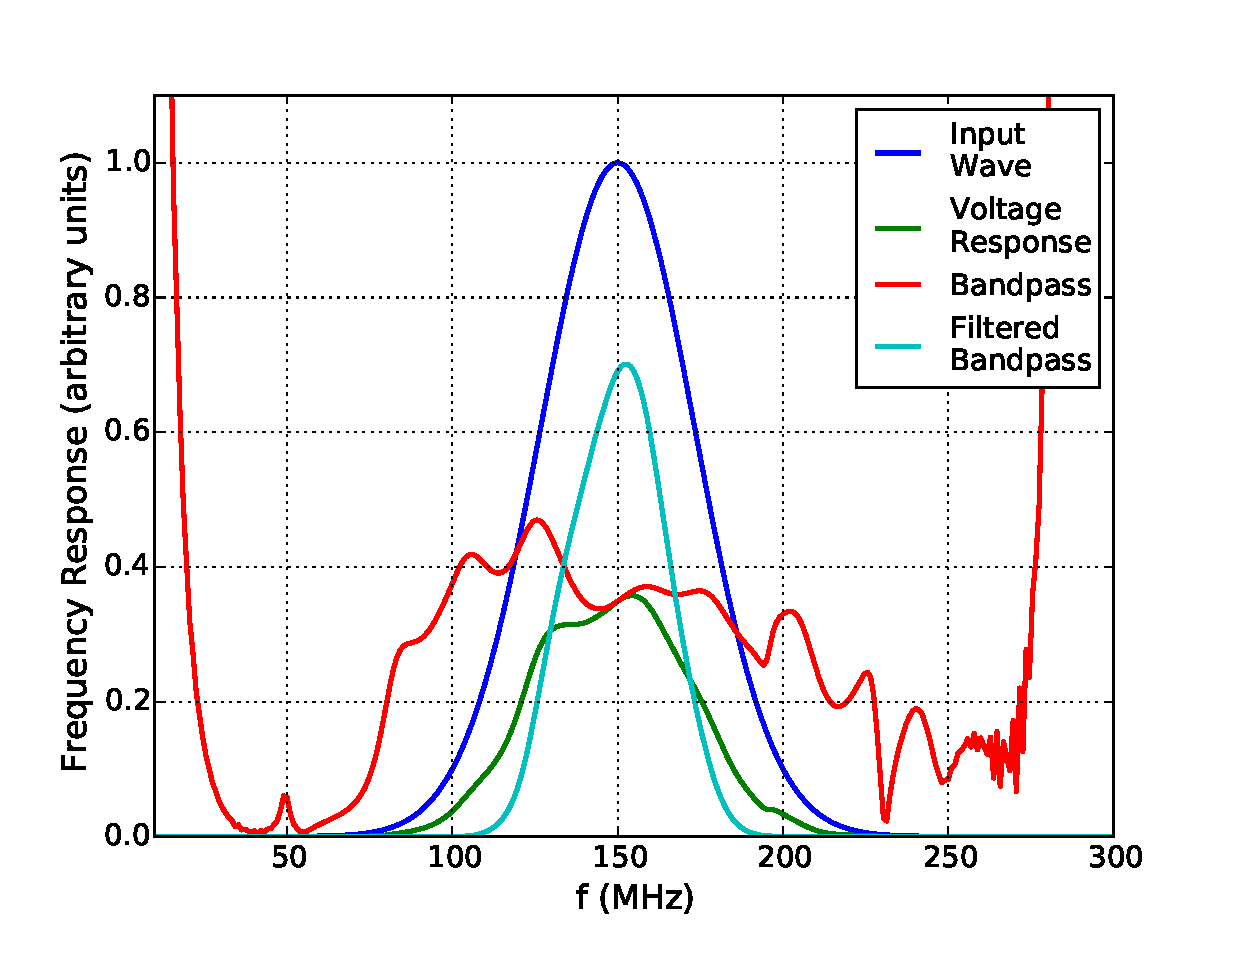
\includegraphics[width=.5\textwidth]{figures/frequency_domain.pdf}
\caption{The absolute value of the discrete Fourier transform of our simulation outputs. We obtain the effective response function of the dish by Fourier transforming the voltage output from our dish (green line) and dividing by the Fourier transform of the input wave (blue line). The simple ratio is plotted as a red line. Since our input is limited to frequencies between $\approx 20$ and $280$\,MHz, there is significant numerical noise that will effect our result outside of this region which we see in the divergene of the red line towards the edges of the plot. To eliminate this noise, we multiply by a Hamming window between $50$ and $250$\,MHz and set our estimate to zero elsewhere. The Fourier transform of our response estimate with the filter applied is shown as a cyan line.}
\label{fig:FrequencyDomain}
\end{figure}

\section{Results and Comparison to Reflectometry Data}\label{sec:Comparison}
\subsection{The Delay Response at Zenith}
In Fig.~\ref{fig:Comparison}, we show the filtered response function deconvolved from our electromagnetic simulations. The response of the dish rapidly dies off as a function of time. After $\approx90$\,ns, we observe lobed structures with a period of $\approx 30$\,ns which corresponds to the geometrical delay between the feed and the dish apex, indicating that the large $\tau$ roll off is dominated by reflections between the feed and the dish. 

Our simulations are intended to verify direct reflectometry measurements taken on a prototype of the HERA feed and dish in Green Bank, presented in \citep{Patra:2015}. For the readers convenience, we briefly explain the reflectometry measurement here before comparing them to our simulation.   

In the reflecometry measurement, a signal is sent from a Vector Network Analyzer (VNA) via a coaxial cable (which is calibrated out) into the back of the feed. The VNA than measures the ratio between returned and transmitted power as a function of frequency, $S_{11}(f)$. A fundamental difference between the reflectometry measurement and the delay response that we are attempting to obtain is that at zero delay, $S_{11}$ is measureing the reflection of the input wave off of the back of the feed while in the delay response of the antenna, the zero delay reflection is the fraction of the electromagnetic wave off of the sky that is accepted by the feed. To obtain $\boldsymbol{\widehat{\rho}}$, we must correct for this difference. It is shown in \citep{Patra:2015} that the correction is 
\begin{equation}
\widehat{\rho}(f) = \frac{\Gamma_a(f)}{1-\Gamma_a(f)} \left[ S_{11}(f) - \Gamma_a(f) \right] + 1 - \Gamma_a(f).
\end{equation}
Applying this transformtion to $S_{11}(f)$ and taking a DFT into the time domain over a band of $100-200$\,MHz, we obtain a measurement based estimate of the dish response function at zenith which is plotted in Fig.~\ref{fig:Comparison} alongside our simulation result. The general trends of the two two lines are in excellent agreement though the phases of the reflections at large time scales are $\approx 10$\,ns out of phase. As the long term delay structure of the delay response determines to what extent foregrounds leak out of the wedge, our simulations verify our measurement of the HERA dish's key performance feature.
\begin{figure}[h!]
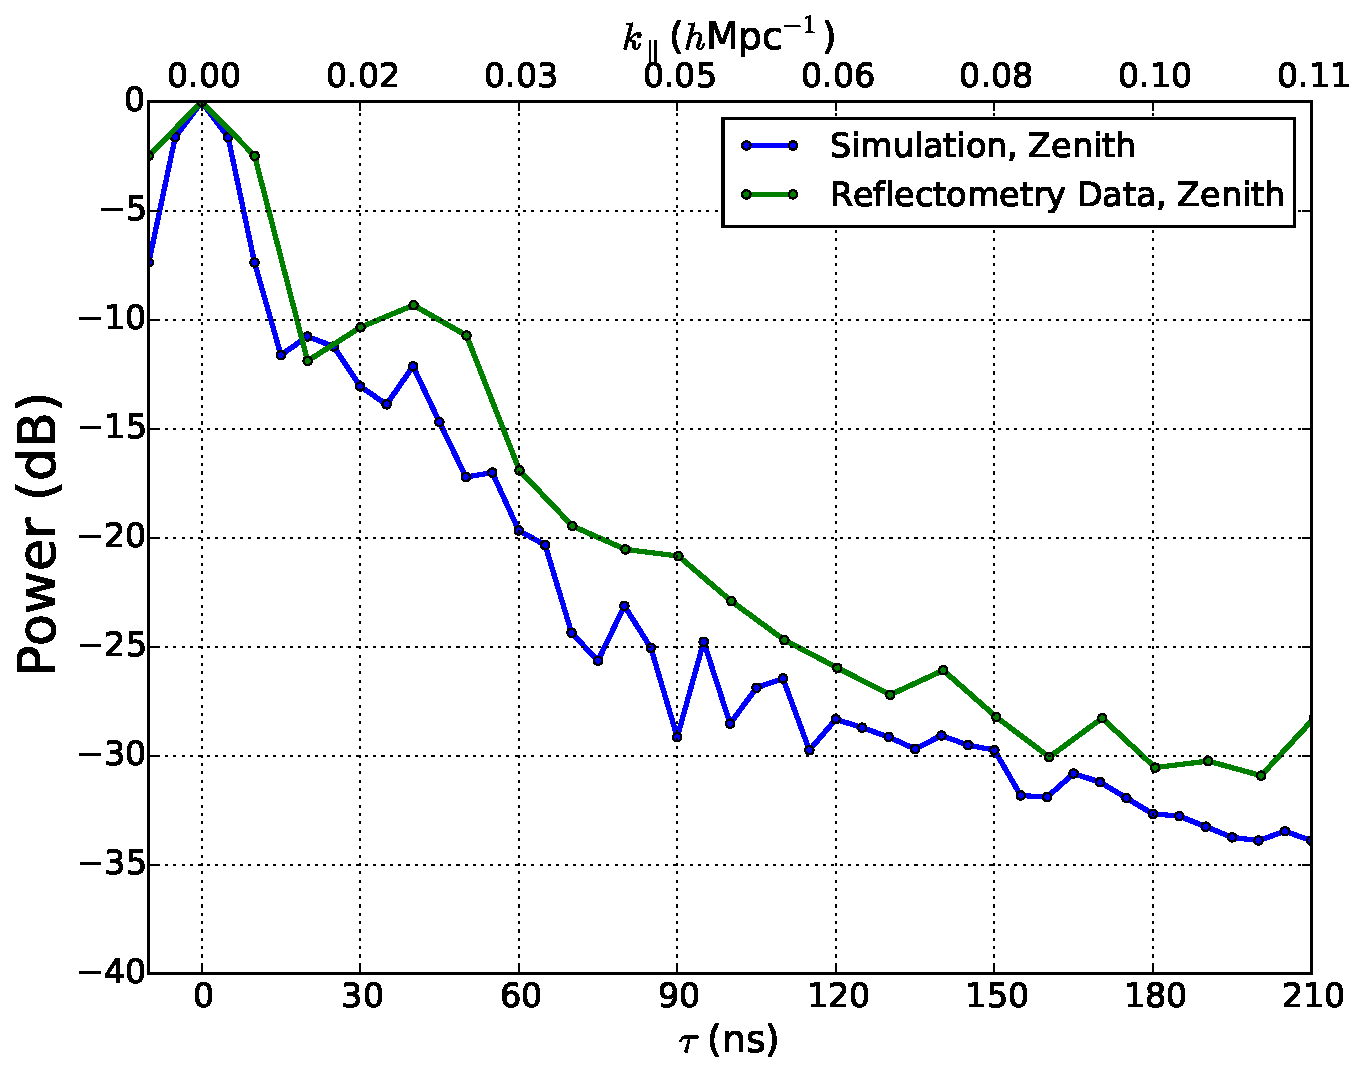
\includegraphics[width=.5\textwidth]{figures/compareSimToDataNormalized.pdf}
\caption{The response function deconvolved from our simulation (blue line) compared to the response function estimated from reflectometry measurements described in \citep{Patra:2015}. Our simulations are in good agreement with the reflectometry results, dropping below $-60$\,dB at $180$\,ns. Since the foregrounds are $\approx 10^6$ times larger than the signal, the necessary attenuation of zenith emission is obtained after $\approx 0.1$\,$h$Mpc$^{-1}$.}
\label{fig:Comparison}
\end{figure}
\subsection{The Delay Response of the Sidelobes}
 After observing decent agreement between simulations and data, we now use our time-domain simulations to probe the side-lobe structure of the dish which are currently inaccessible to our experimental setup. Understanding the delay structure of the sidelobes is critical for several reasons. First, the sidelobes represent the largest delays occupied by foregrounds, hence the closest to the EoR window which we wish to keep foreground-free. While spectral leakage of sources at zenith may place them somewhere within the wedge, any spectral structure in the sidelobes is guaranteed to place these sources directly inside of the window. Second, the forshortening of diffuse structure near the horizon due to wide-field projection effects leads to a significant amount of foreground power entering at these delays, generally making them the most contaminated region of the wedge outside of the central lobe and leading to the so called ``pitchfork" \citep{Thyagarajan:2015a,Thyagarajan:2015b}. 
 
 We fist attempt to explore the Dish sidelobe structure by running high resolution spatial beam maps {\bf Rich fill in details of running 2D beam simulations}. However, comparison between individual frequency channels in both CST and FEKO indicates numerical precision errors {\bf Show a figure of an attempted beam and frequency artifacts at zenith.}


\section{The Effect of the HERA dish Chromaticity on Foreground Leakage and Sensitivity}\label{sec:Foregrounds}

\subsection{Simulating Foreground Visibilities with the Spectral Structure of the HERA Dish.}

\subsection{How Deep Can we Clean?}
The level of foreground subtraction possible depends on the number of time steps and redundant baselines that are averaged before performing the cleaning step. The standard deviation on the real and imaginary part of a single delay transformed visibility is given by \citep{Morales:2004}
\begin{equation}
\Delta V = \frac{\sqrt{2 B} k_B T_{sys}}{A_e \sqrt{\tau}}
\end{equation}
where $A_e$ is the effective area of the dish, $B$ is the bandwidth, $T_{sys}$ is the system temperature, $\tau$ is the integration time, and $k_B$ is the Boltzmann constant. The system temperature can be calculated by assuming that $T_{sys} = 100\text{K} + T_{sky}$ where $100$\,K is the temperature of the PAPER reciever and $T_{sky} = 60 (\lambda/1\,\text{meter} )^{2.55}$ is the sky temperature \citep{Fixsen:2008}. For $A_e$ we use the value of $75$\,m determined in \citep{Neben:2015b}. If we assume that each baseline is cleaned independently and that the integration time is $\tau \approx 60$\,s, than the noise level at 150\,MHz is approximately $9.9$\,Jy\,MHz. In order to avoid subtracting noise, we assume that cleaning is performed down to $5\,\sigma$. In Fig.~\ref{fig:Cleaning}, we see that cleaning to $5\,\sigma$ 

\begin{figure}
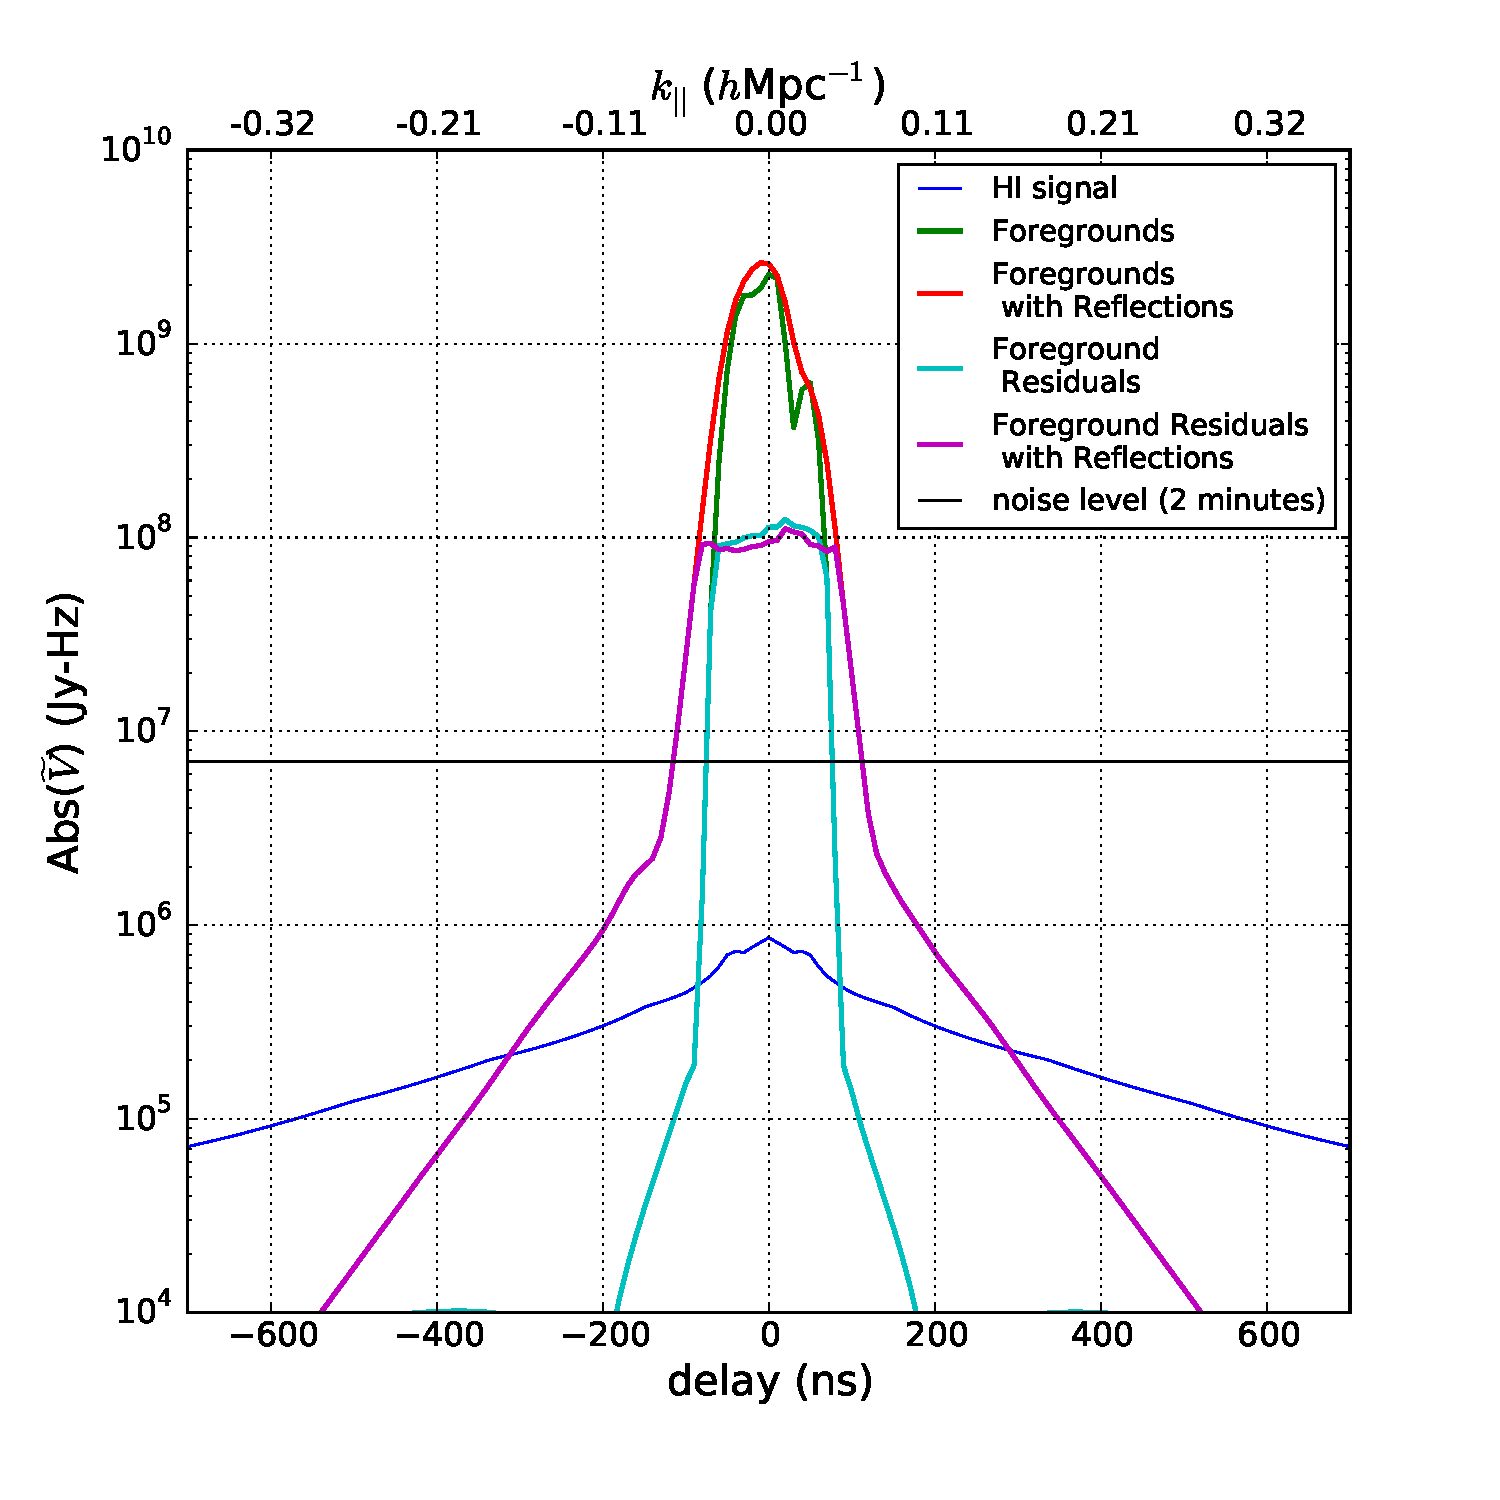
\includegraphics[width=.5\textwidth]{figures/cleaning_noise.pdf}
\caption{The absolute magnitude of a delay transformed 14-meter baseline (blue line) compared to the same visibility (green line) contaminated by reflections at the level observed in the HERA dish design. We see that the extended delay kernel smooths out structure, originating from foregrounds, within the horizon. For HERA, we expect to use the delay-clean to remove foregrounds. However, the depth of cleaning is limited by the noise level on a single baseline (black line). We show the foreground residuals with arising from a clean down to the $5\,\sigma$ noise level after 2 minutes of integration, seeing that cleaning at this cadence achieves $\approx$ two orders of magnitude of foreground reduction. The reflections in the dish lead to extensive winged structures that bleed into the EoR window and are well below the thermal noise level. All data in this plot are obtained from a $100$\,MHz bandwidth centered at $150$\,MHz.}
\label{fig:Cleaning}
\end{figure}


\begin{figure}
\centering
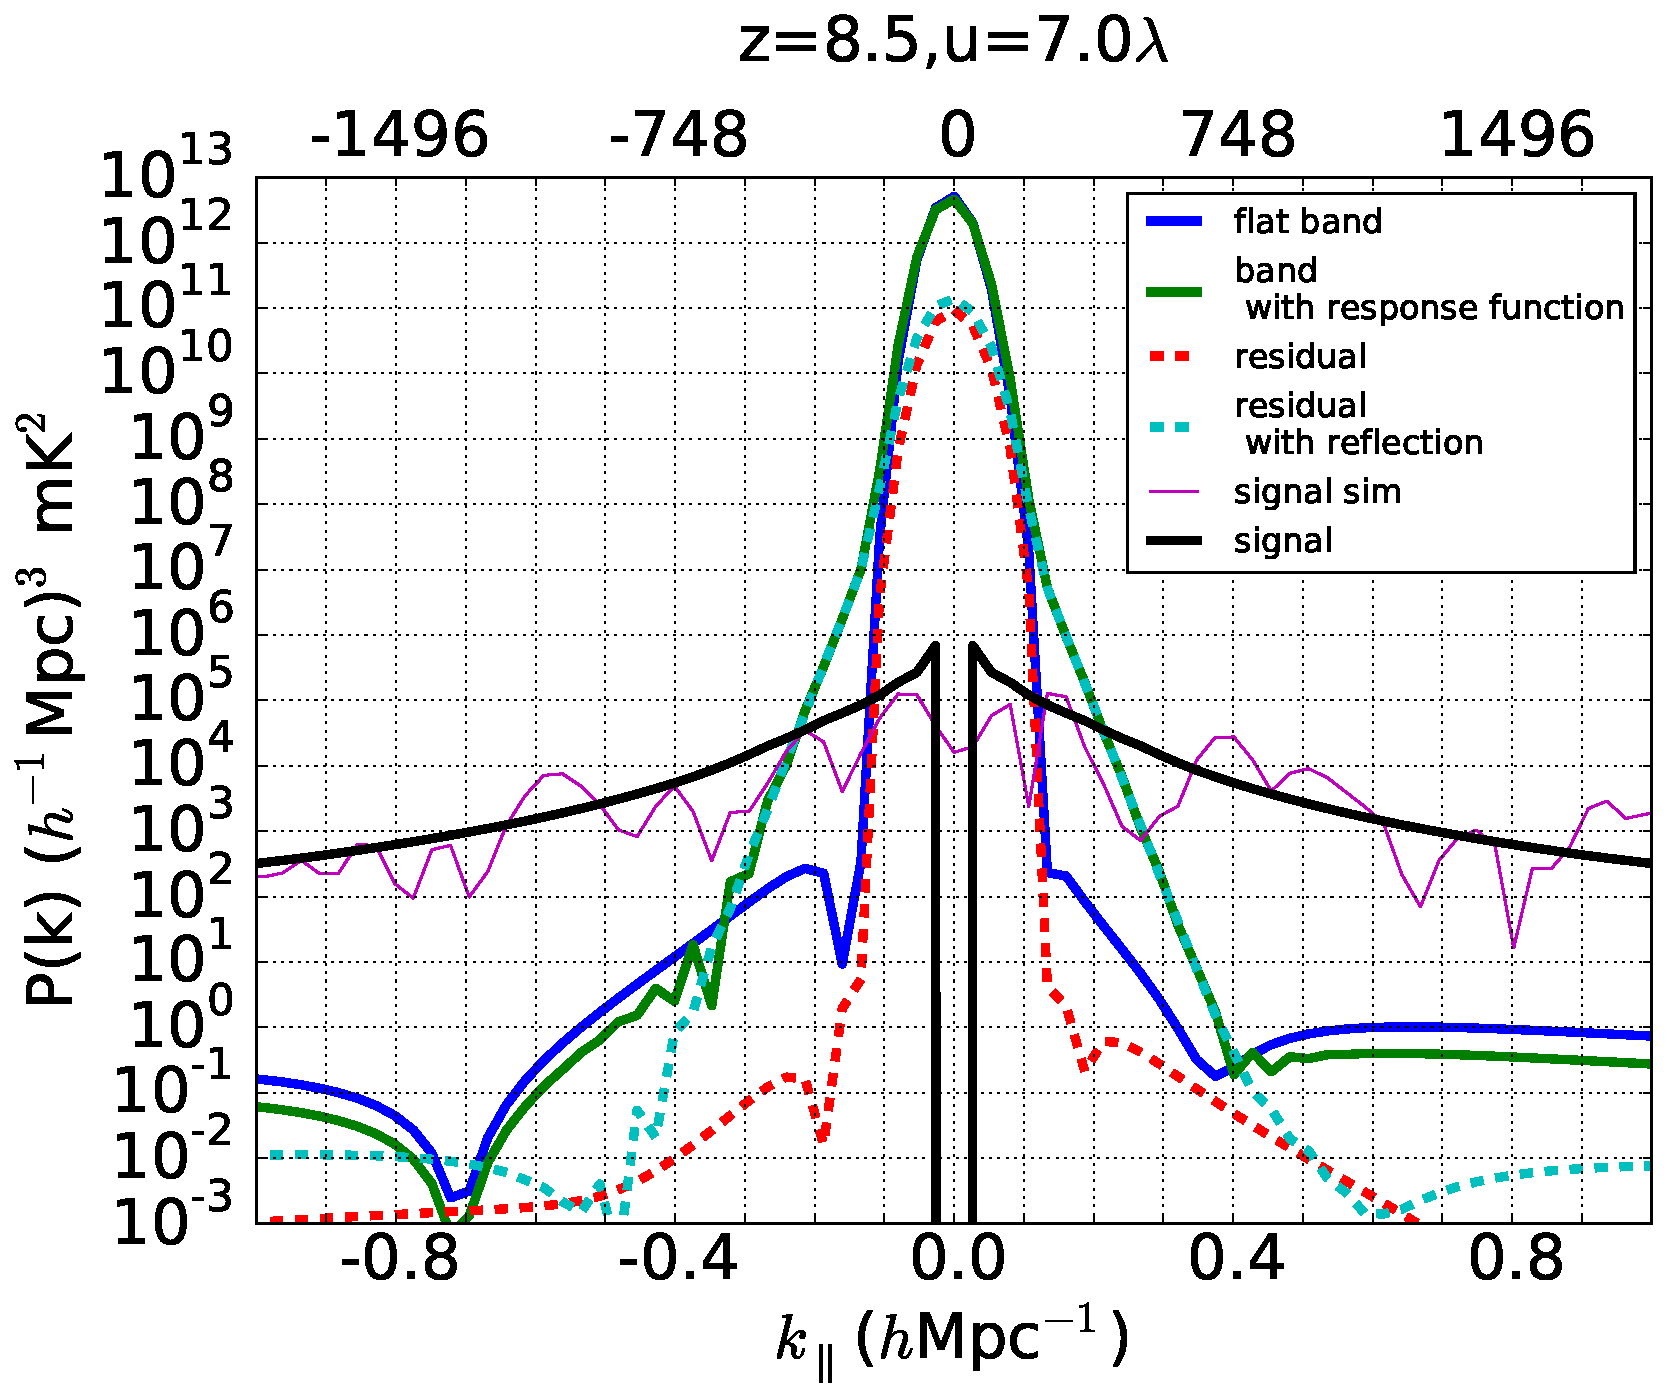
\includegraphics[width=.5\textwidth]{figures/resid_5sigma_compare.pdf}
\caption{The delay transformed power spectra of foregrounds with (blue line) and without (green line) contamination from reflections in the dish. The residuals of these foregrounds, cleaned to $5\,\sigma$ after 2 minutes of integration, are plotted with (red dashed line) and without (cyan dashed line) dish reflections. We compare to the amplitude of the 21\,cm power spectrum (solid black line). Foreground contamination, leaked by reflections, extends out to $k_\parallel \approx 0.25$\,$h$Mpc$^{-1}$. The signals plummet to zero at $k=0$ is an artifact of the spatial extent of the simulation which does not probe extremely fine scales.}
\label{fig:SignalCompare}
\end{figure}

\subsection{The Implications of Dish Reflections on EoR Science}
Since the amplitude of the 21\,cm signal is maximal at smaller $k$ values, a loss of large scale signal out to $0.25$\,$h$Mpc$^{-1}$ will eliminate some of the power spectrum modes that HERA will have the greatest SNR on, impacting our overall sensitivity. We address the change in SNR and its implications on HERA's ability to place constraints on reionization parameters in this section, using the Fisher Matrix Formalism. 



\begin{figure}
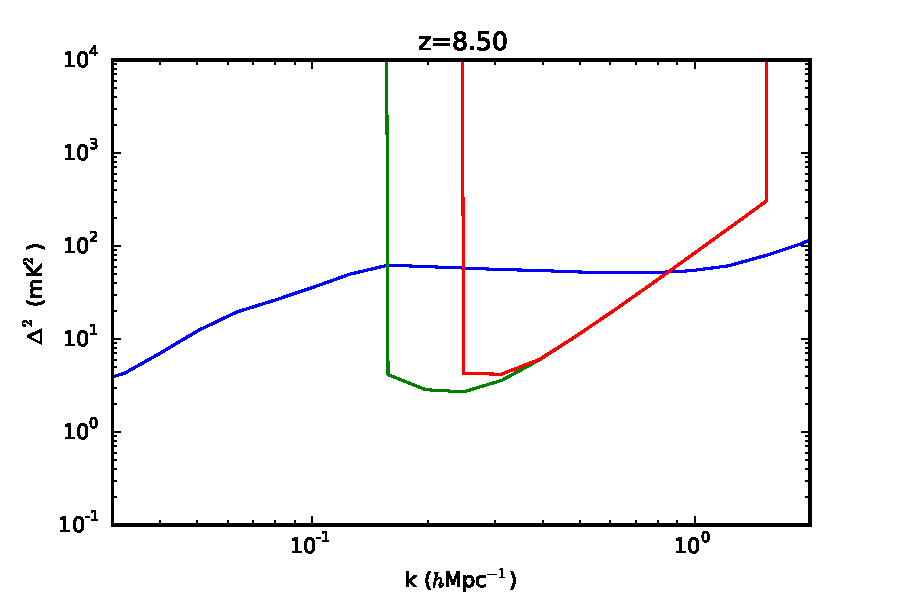
\includegraphics[width=.5\textwidth]{figures/sensitivity_comparison.pdf}
\caption{Comparison between sensitivities with and without reflections.}
\end{figure}


\begin{figure}
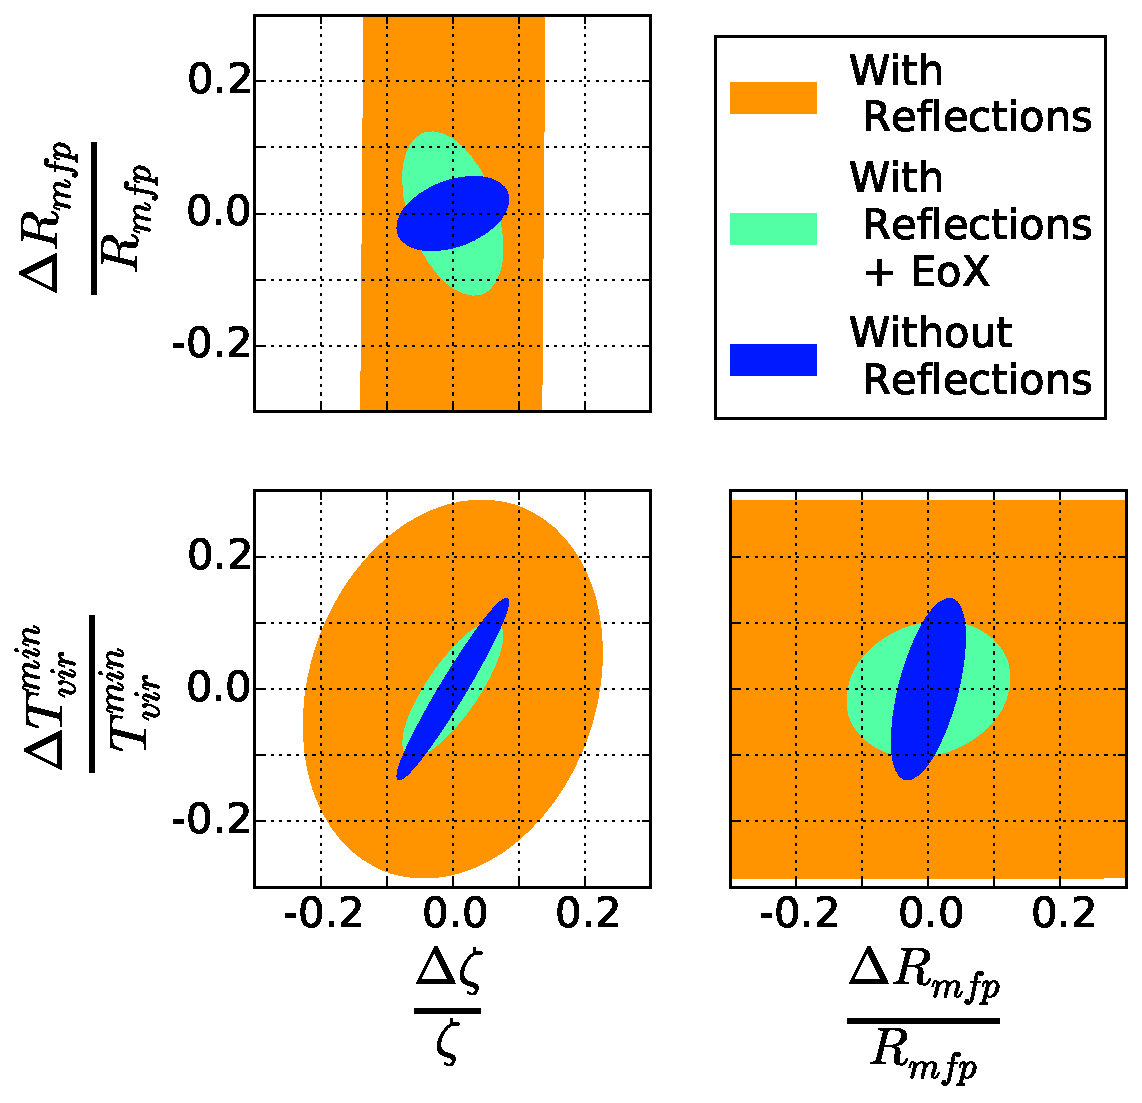
\includegraphics[width=.5\textwidth]{figures/reionization_triangle_compare.pdf}
\caption{95\% confidence interfals with and without reflections. The primary effect of a large minimal delay accessible is that  the ``knee" which is the primary lever on $R_\text{mfp}$ becomes inaccessible at low redshift. Since the comoving minimal $k$ corresponding to a minimal delay becomes smaller at higher redshift, EoX measurements do improve constraints on $R_\text{mfp}$. }
\end{figure}


\begin{figure*}
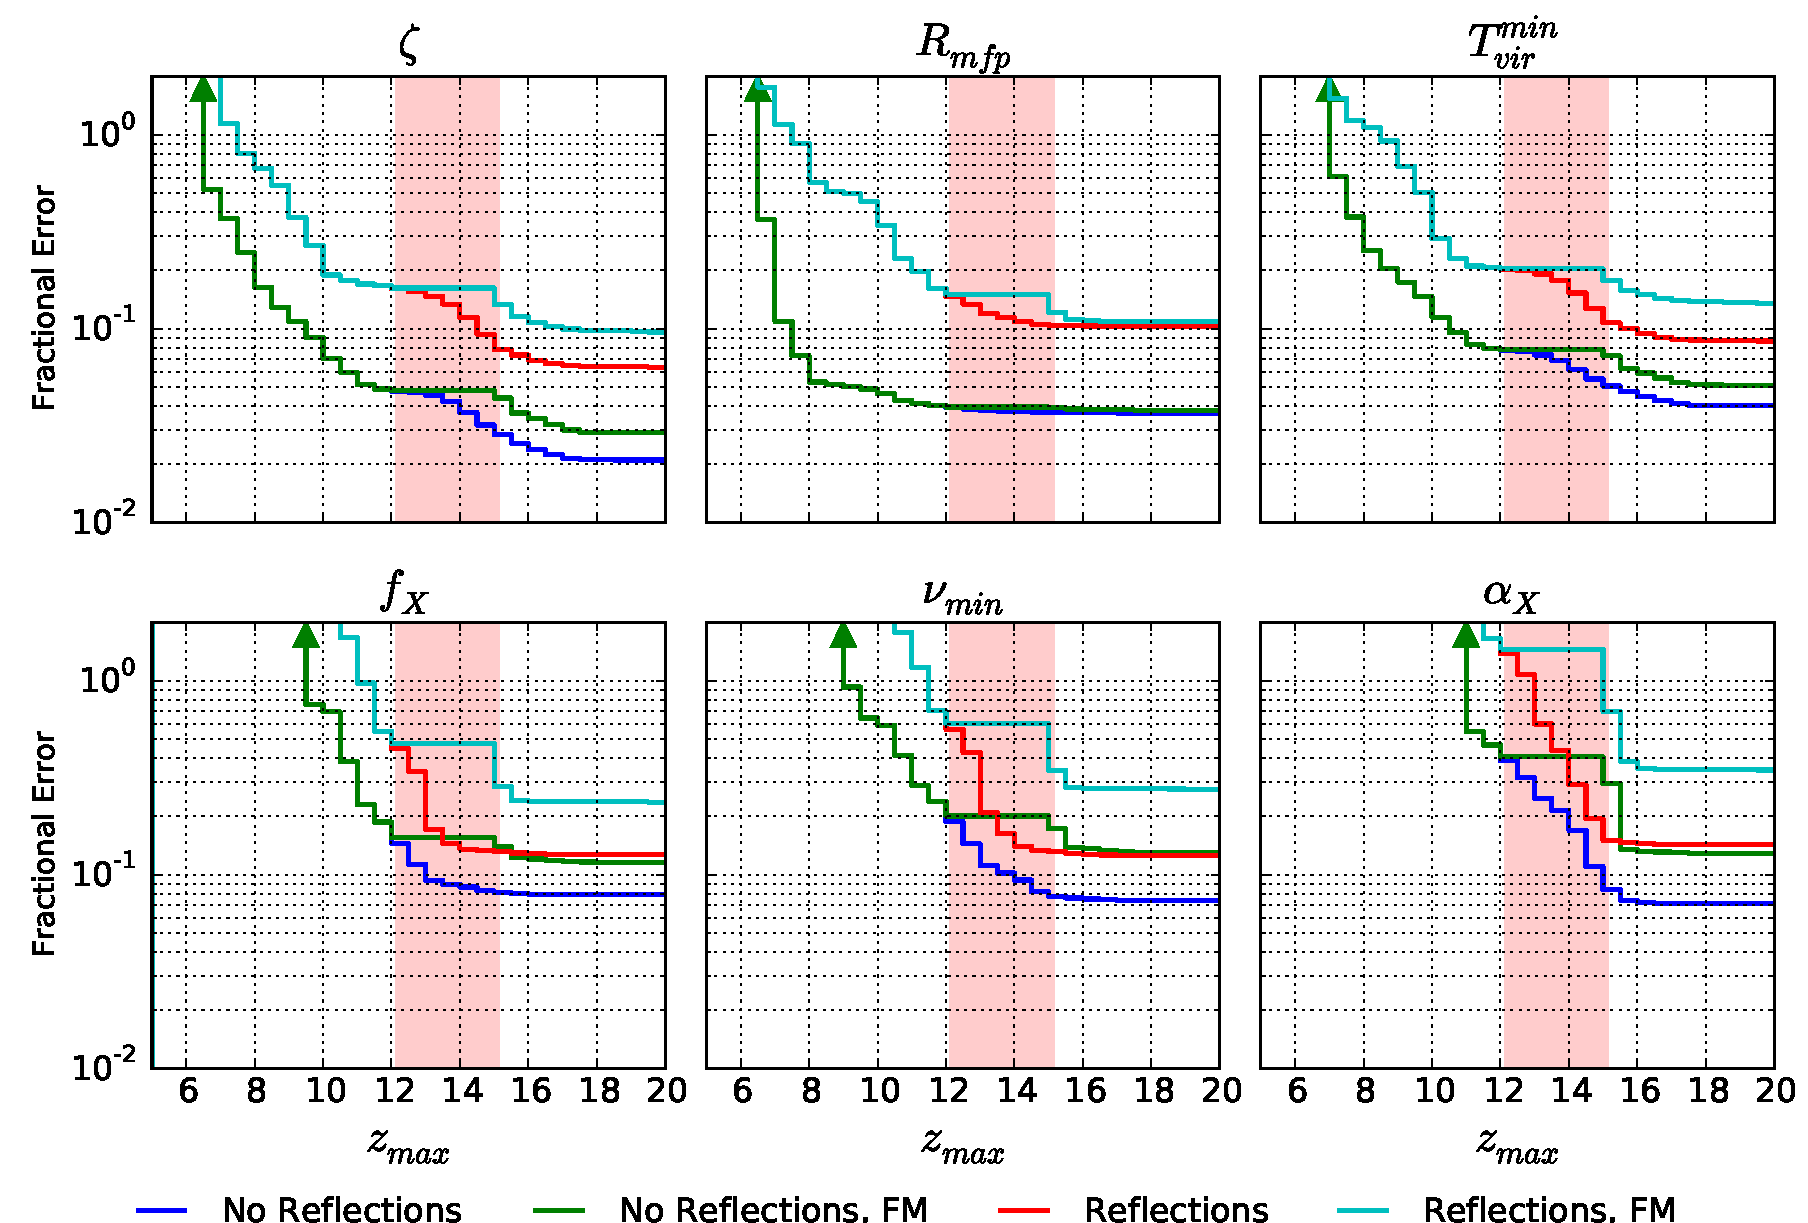
\includegraphics[width=\textwidth]{figures/sigmaVsZ.pdf}
\caption{Fractional Errors on reionization and heating parameters as a function of maximal observed redshift.}
\end{figure*}

\begin{figure}
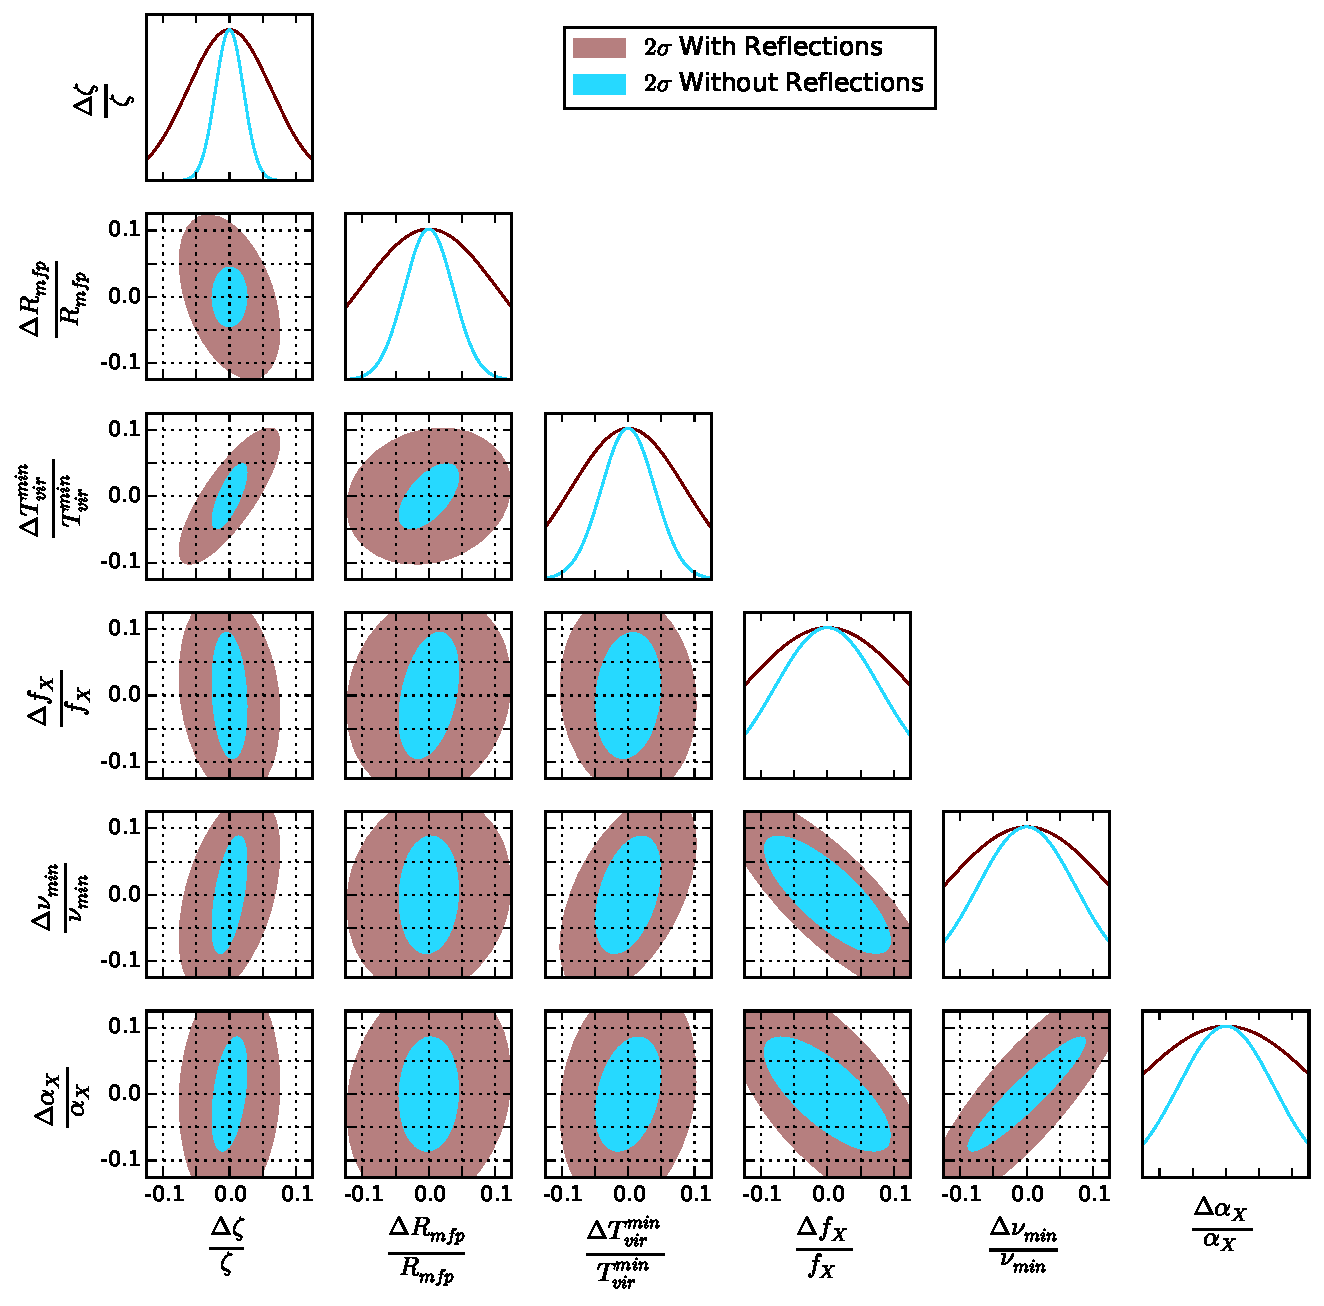
\includegraphics[width=\textwidth]{figures/triangle_hera331.pdf}
\caption{95\% confidence regions with and without reflections assuming that observations are taken over the redshifts between 5 and 25 are observed.}
\end{figure}


\section{Conclusions}
\label{sec:Conclusion}
\bibliographystyle{apj}
\bibliography{DishSimulation_paper_v0}

\appendix
\section{The Effect of Reflections and Cross-Talk on Visibilities}\label{app:Reflections}
In this section, we investigate, formally, the impact of reflections of electromagnetic waves between antennas and within the signal chain of single antennas on foreground leakage in 21\,cm experiments. We start with the time varying electric field from a single source with location ${\bf \widehat{k}}$ on the sky, arriving at antenna $i$ with delay $\tau_i$ and antenna $j$ with delay $\tau_j$ with respect to the electric field at the origin which we denote as $s(t,{\bf \widehat{s}})$. We allow for two different types of reflections: First, we allow reflections within the analogue path of each $i^{th}$ antenna which we denote as $r_i(\tau,{\bf \widehat{s}})$. We also allow for single reflections between any $i-j$ antenna pair which we denote as $r_{ij}(\tau',{\bf \widehat{s}})$. Our choice of arbitrary $\tau'$, for now, allows for multi-path propogation between antennas, though we expect it to be dominated by the geometrical delay between the antenna pair. The electric field at antenna $i$ is given by
\begin{equation}
s_i(t,{\bf \widehat{s}}) = \int d \tau' r_i(\tau',{\bf \widehat{s}})s(t+\tau_i-\tau') + \sum_{j \ne i} \int d \tau' s(t + \tau_j - \tau_{ij}) r_{ij}(\tau',{\bf \widehat{s}})
\end{equation}  
In an FX correlator, the electric field is sampled, Fourier transformed, and cross multipled between antenna pairs to form visibilities. The Fourier transform step leaves us with 
\begin{equation}
\widetilde{s}_i(f,{\bf \widehat{s}}) = \widetilde{s}(f,{\bf \widehat{s}}) \left[ \int d \tau' r_i(\tau',{\bf \widehat{s}})e^{2 \pi i(\tau_i - \tau')f} + \sum_{j\ne i} \int d \tau' e^{2 \pi i(\tau_j - \tau_{ij})f} r_{ij}(\tau',{\bf \widehat{s}}) \right]
\end{equation}
Multiplying and averaging gives us the visibility for the single source we obtain
\begin{align}\label{eq:SingleSource}
v_{ij}'(f,{\bf \widehat{s}}) & = \langle \widetilde{s}_i(f,{\bf \widehat{k}}) \widetilde{s}_j(f,{\bf \widehat{s}}) \rangle_t \nonumber \\
&=d \Omega  I(f,{\bf \widehat{s}}) g_i(f) g_j^*(f) a_i(f,{\bf \widehat{s}})a_j^*(f,{\bf \widehat{s}}) e^{2 \pi i{\bf u_{ij}} \cdot {\bf \widehat{s}}} + d \Omega I(f,{\bf \widehat{s}}) \sum_{\ell \ne j} g_i(f)a_i(f,{\bf \widehat{s}}) C_{\ell j}^*(f,{\bf \widehat{s}}) e^{2 \pi i {\bf u_{\ell i} \cdot {\bf \widehat{s}}}} \nonumber \\ 
& + d \Omega I(f,{\bf \widehat{s}})\sum_{k \ne i} g_j^*(f) a_j^*(f) C_{ki}(f,{\bf \widehat{s}}) e^{2 \pi i {\bf u_{kj}\cdot {\bf \widehat{s}}}} + d \Omega I(f,{\bf \widehat{s}}) \sum_{k\ne i}\sum_{\ell \ne j} C_{ki}(f,{\bf \widehat{s}}) C_{j\ell}^*(f,{\bf \widehat{s}}) e^{2 \pi i {\bf u_{k\ell}}\cdot{\bf \widehat{s}}},
\end{align}
where $g_i(f) a_i(f,{\bf \widehat{s}}) = \int d \tau r_i(\tau,{\bf \widehat{s}}) e^{2 \pi i f \tau}$ is the effective direction dependent gain of the system which can be factored into a directoin dependent and direction independent function where $g_i(f)$ is the gain of the analogue signal chain after the radiation has been absorbed by the feed and $a_i(f,{\bf \widehat{s}})$ describes the chromatic electric field response of the antenna. The first term in equation~\ref{eq:SingleSource} is an effective visibility with self-reflections. The two cross terms and the last term involve the mixing of visibilities complementary too the $ij$ baseline and have the potential to introduce significant chromatic features since they potentially insert visibilities on much longer basline lengths. Assuming propogation along a single path directly between the antennas, we may write $C_{ik}(f,{\bf \widehat{s}})$ as 
\begin{equation}
C_{ki}(f,{\bf \widehat{s}}) = a_i(f,{\bf \widehat{s}}_{ki}) \frac{1}{r_{ik}}\left[\frac{d \sigma_k}{d \Omega}(f,{\bf \widehat{s}},{\bf \widehat{s}}_{ik})\right]^{1/2} e^{2 \pi i \tau_{ik} f}
\end{equation}
Where $r_{ik}$ is the distance between antennas $i$ and $k$, $d \sigma_k (f,{\bf \widehat{s}},{\bf \widehat{s}}_{ij})/ d \Omega $ is the cross-section of the antenna to scatter radiation from the ${\bf \widehat{s}}$ direction to the ${\bf \widehat{s}}_{ik}$ direction where ${\bf \widehat{s}}_{ik}$ is the unit vector in the direction between antenna $i$ and antenna $k$. Integrating over the primary beam, we obtain a full expression on the effect of the foregrounds. 
\begin{align}
V_{ij}' = \int d \Omega v_{ij}'(f,{\bf \widehat{s}}) &= g_i(f) g_j(f)^* \int d \Omega A_{ij}(f,{\bf \widehat{s}}) I(f,{\bf \widehat{s}})e^{2 \pi i f {\bf u_{ij}} \cdot {\bf \widehat{s}}} + g_i(f) \sum_{\ell \ne j} \int d \Omega  A_{i\ell j}(f,{\bf \widehat{s}}) I(f,{\bf \widehat{s}})e^{2 \pi i {\bf u_{\ell i} } \cdot {\bf \widehat{s}} } \nonumber \\ 
& + g_j^*(f) \sum_{k \ne i}  \int d \Omega A^*_{jki}(f,{\bf \widehat{s}}) I({\bf \widehat{s}},f) e^{2 \pi i {\bf u}_{kj} \cdot {\bf \widehat{s}} } + \sum_{k \ne i} \sum_{\ell \ne j}\int d \Omega A_{k i \ell j}(f,{\bf \widehat{s}}) I(f,{\bf \widehat{s}})e^{2 \pi i {\bf u}_{k\ell} \cdot {\bf \widehat{s}}}
\end{align}
which is essentially an ad-mixture of many baselines with different effective primary beams. We denote the effective primary beam of the $i,j$ antenna pair as $A_{ij}(f,{\bf \widehat{s}})=a_i(f,{\bf \widehat{s}})a_j^*(f,{\bf \widehat{s}})$, the effective beam from a single reflection correlated with a direct measurement as $A_{i \ell j} = a_i(f,{\bf \widehat{s}}) C^*_{\ell j}(f,{\bf \widehat{s}})$ and the correlation between entirely reflected terms as experiencing an effective primary beam of $A_{k i \ell j}=C_{ki}(f,{\bf \widehat{s}}) C^*_{j \ell}(f,{\bf \widehat{s}})$. In this paper, we focus on the reflection terms within a single antenna element. Hence, we ignore all but the first term for now. Any reflection terms occurring downstream of the conversion by the feed from electromagnetic radiation to voltage are lumped into $g_i(f)$ and reflections occurring within the antenna element enter into $a_i(f,{\bf \widehat{s}})$. While reflections within the analogue system are a potential source of contamination, HERA's post-feed analogue signal path is designed to keep all reflections under 35\,m, within the wedge. 

The focus of this paper and its companions is the reflection properties of the primary antenna element, so we will focus the rest of our discussion here on $a_i(f,{\bf \widehat{s}})$. The primary elements of our dish include a feed and backplane suspended over a fourteen meter dish. We assume a set of discrete reflections within the dish, which without loss of generality are assumed to have frequency independent reflection coefficients\footnote{If we allow each coefficient to be frequency dependent, we can expand each frequency dependent term in a Fourier series of frequency independent terms} hence 
\begin{equation}
a_i(f,{\bf \widehat{s}}) = \sum_{n} r_n({\bf \widehat{s}}) e^{2 \pi i  \tau_n f}
\end{equation}
Assuming all antennas are identical, we have
\begin{equation}
A_{ij}(f,{\bf \widehat{s}}) = \sum_m \sum_n r_n({\bf \widehat{s}}) r_m^*({\bf \widehat{s}}) e^{2 \pi i(\tau_n-\tau_m)f} = \sum_\alpha A_\alpha({\bf \widehat{s}}) e^{2 \pi i \tau_\alpha}
\end{equation}
where we have re-indexed $m$ and $n$ under a single greek index $\alpha$ in the second equality. The effect of internal reflections on a visibility is hence
\begin{equation}
V_{ij}'= \sum_\alpha \int d \Omega A_\alpha({\bf \widehat{s}}) e^{2 \pi i \tau_\alpha f} e^{2 \pi i {\bf b}_{ij} \cdot {\bf \widehat{s}}f/c} I(f,{\bf \widehat{s}})
\end{equation}
Taking the delay transform, one obtains
\begin{equation}
\widetilde{V}_{ij}'(\tau) = \sum_\alpha \widetilde{V}_{ij}^\alpha (\tau - \tau_\alpha)
\end{equation}
where 
\begin{equation}
\widetilde{V}^\alpha_{ij}(\tau) = \int d \tau e^{-2 \pi i f \tau} \int d \Omega A_\alpha({\bf \widehat{s}}) e^{2 \pi i {\bf b}_{ij} \cdot {\bf \widehat{s}} f/c} I(f,{\bf \widehat{s}})
\end{equation}
is the usual delay transform of \citet{Parsons:2012}. $\widetilde{V}_{ij}^alpha(\tau)$.
\end{document}